\chapter{推荐系统}

\section{召回模型}

\subsection{协同过滤 (Collaborative Filtering)}

\subsection{Embedding召回方法}

\subsubsection{KD-Tree 算法}

\textcolor{importcolor}{\bfseries KD-Tree构建}:选择高维向量中的某一维(一般采用轮转的方式),将当前结点上的数据点按照这些数据点在该维度上的中位数进行划分,重复上述过程直到树的结点不包含数据点为止。

\textcolor{importcolor}{\bfseries KD-Tree检索}:1) 首先由树的根结点寻到目标点所在的叶子结点,并以当前叶子结点作为最近邻的候选点;2) 递归地判断当前结点的兄弟结点是否与以目标点为中心,以当前最短距离为半径的超球体相交;3)如果相交则进入兄弟结点进行搜索,搜索过程对最短距离进行实时更新;如果不相交则往父结点回退直到回退到根结点终止。

\begin{note}
  读者朋友如果希望通过例子来更加直观理解KD-Tree的检索过程,可以参考\href{https://zhuanlan.zhihu.com/p/23966698}{KD树算法之详细篇}。KD-Tree检索K近邻与检索最近邻类似,只需在检索过程中维护一个存储当前K近邻的list或者大顶堆即可。
\end{note}

\subsubsection{局部敏感哈希(Local Sensitive Hash)}

局部敏感哈希的基本思路是:两个高维空间上距离近的点,映射到低维空间中的两个投影点也相对靠近;两个高维空间上距离较远的点,映射到低维空间中的投影则可能较远也可能较近。那么,如果我们随机构建若干投影映射,如果两个点在多个投影映射下的投影点都有相近的距离,那么大概率这两个点在原始空间中也距离较近。

我们可以假设有$N$个投影映射$\{(\bm{p}_1,b_1),(\bm{p}_2,b_2),\dots,(\bm{p}_N, b_N)\}$,且对应的分桶宽度为$\{w_1,w_2,\dots,w_N\}$,那么对于高维空间中的向量$\bm{x}$,落在映射$i$的分桶为:
\begin{equation}
  h_i(\bm{x})= \lfloor \frac{\bm{p}_i^T + b_i}{w_i} \rfloor
\end{equation}
其中,$h_i(\bm{x})\in \mathbb{Z}$为分桶标号。对于高维空间中的两个点$\bm{x}_1,\bm{x}_2$,如果各自的分桶标号$(h_1(\bm{x}_1), h_2(\bm{x}_1),\dots,h_N(\bm{x}_1))$和$(h_1(\bm{x}_2), h_2(\bm{x}_2),\dots,h_N(\bm{x}_2))$在大多数维度上重合,则$\bm{x}_1,\bm{x}_2$在原始空间中相近。

\begin{note}
  关于局部敏感哈希的详细介绍,可以参见Pinecore的\href{https://www.pinecone.io/learn/series/faiss/locality-sensitive-hashing/}{Locality Sensitive Hashing: The Illustrated Guide}。
\end{note}

\subsubsection{Hierachical Navigable Small Worlds (HNSW)}

HNSW 算法构建了一个分层的索引图,如图\ref{fig:hnsw}所示\footnote{图片来源于Pinecone。}。位于上层的索引图较为“稀疏”,点与点之间有较大距离。越往下层,索引图越“稠密”,点与点之间的距离则更近。在搜索时,先从上层索引进行搜索,找到近似最近邻点,再跳转至下层对应的点,并重复搜索过程,直到在最底层的索引图上找到最近邻点。HNSW 算法构建索引图以及在索引图上搜索的详细过程请参见 \href{https://www.pinecone.io/learn/series/faiss/hnsw/}{Hierachical Navigable Small Worlds}。

HNSW 索引是工业场景中最受欢迎的索引方法之一,尤其适合索引规模特别庞大的场景(Billion级别甚至更大),但构建该索引过程较为耗时,且会占用大量的存储空间。

\begin{figure}[htbp]
  \centering
  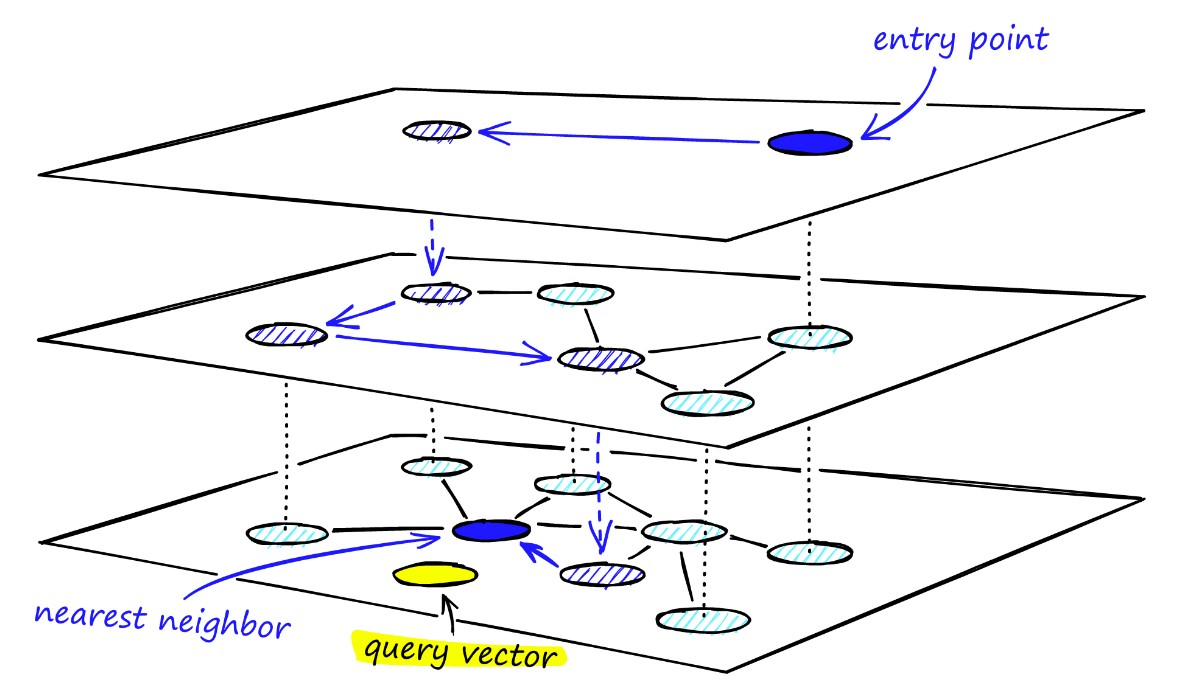
\includegraphics[width=0.6\textwidth]{hnsw.jpg}
  \caption{HNSW检索最近邻过程 \label{fig:hnsw}}
\end{figure}


\section{粗排与精排}